\documentclass{article}

\usepackage{amsmath,amssymb,amsfonts}
\usepackage{thmtools,thm-restate}
\usepackage[thmmarks,amsmath]{ntheorem}
\usepackage{mathtools}
\usepackage[utf8]{inputenc}

\usepackage[toc,title]{appendix}

\usepackage{diffcoeff}
\diffdef{}{op-symbol=\mathrm{d},op-order-sep=0mu}
\usepackage[integrals]{wasysym}

\usepackage{cancel}
\usepackage{braket}

\usepackage{tikz}

\usepackage{cite}

%\usepackage[portuges]{babel}

\title{Project in Calculus of Variations\\
\large Holonomic and Non-Holonomic Constraints, with Lagrange Multipliers}
\author{Duarte Maia}
\date{May 2021}

\theoremstyle{plain}
\theoremseparator{.}
\newtheorem{prop}{Proposition}
\newtheorem{lemma}{Lemma}
\newtheorem{theorem}{Theorem}


\theoremstyle{plain}
\theorembodyfont{\upshape}
\newtheorem{remark}{Remark}
\newtheorem{example}{Example}

\theoremstyle{nonumberplain}
\theorembodyfont{\upshape}
\theoremseparator{.}
\newtheorem{statement}{Problem Statement}
\theoremsymbol{\ensuremath{\blacksquare}}
\newtheorem{proof}{Proof}

\theoremstyle{empty}
\theorembodyfont{\upshape}
\theoremseparator{.}
\theoremsymbol{\ensuremath{\blacksquare}}
\newtheorem{proofref}{Proof}

\newcommand{\R}{\mathbb{R}}
\newcommand{\N}{\mathbb{N}}

\newcommand{\tr}{\intercal}

\newcommand{\tstart}{\mathrm{start}}
\newcommand{\tend}{\mathrm{end}}

\newcommand{\wtphi}{
  \mspace{2mu}
  \widetilde{\mspace{-2mu}\smash[t]{\phi}}
}

\DeclarePairedDelimiter\abs{\lvert}{\rvert}
\DeclarePairedDelimiter\norm{\lVert}{\rVert}
\DeclarePairedDelimiter\eval{.}{\rvert}
\DeclarePairedDelimiter\bracket{[}{]}

\DeclareMathOperator{\tg}{tg}
\DeclareMathOperator{\supp}{supp}

\newcommand{\vecb}{{\bar{b}}}

\begin{document}
\maketitle

\section{Introduction}

This work originally started as a project for a class on the Calculus of Variations, at Instituto Superior Técnico. The topic of the project is classical optimization with holonomic and non-holonomic constraints. However, when doing research on the subject, I was shocked to find very few mathematical references with the Lagrange multiplier theorem for the non-holonomic case, and corresponding proof. Consequently, I have taken it upon myself to create such a reference.

This document is divided into two parts. The first part is a relatively simple exploration of holonomic constraints, that is, optimization on (possibly time-dependent) manifolds. In other words, we require that our paths satisfy equations of the form $\phi_i(t, u(t)) = 0$, $i = 1, \dots, k$. The second part is trickier, in which the restrictions become differential equations of the form $\phi_i(t,u(t), \dot u(t))$, $i = 1, \dots k$. This is where I had a problem finding references.

This work is the culmination of a couple of weeks spent interpreting 16 pages' worth of Bliss' \textit{Lectures on the Calculus of Variations} \cite[pp.~187-202]{bliss}. I don't know whether to blame my unfamiliarity with the notational conventions, the great amount of generality in which the proof is done, or my own lack of experience with the topic, but it was with more effort than I am proud to admit that I could finally understand the proof which I reproduce in section \ref{sec:nonholonomic}, albeit in much less generality (though the essential ideas are there). Perhaps this work might serve as a primer for someone else's reading of Bliss' proof.

\section{Notational Conventions}

In this section we lay down the basic notational conventions that will be followed over the rest of this document.

The problem at hand is to find a curve $u \colon [t_\tstart, t_\tend] \to \R^n$ that minimizes the value of a certain integral $I(u) = \int_{t_\tstart}^{t_\tend} f(t, u(t), \dot u(t)) \dl2 t$. In order for this expression to make sense, it is assumed that the curves $u$ being considered are at least $C^1$, and the function $f$ is at least continuous, though the results to be obtained require in fact that $f$ is at least $C^2$.

The function $f$ is considered to be a function of 3 variables: time $t \in [t_\tstart, t_\tend]$, position $u \in \R^n$ and velocity $\xi \in \R^n$. In truth, we could be considering $f$ defined in more general (i.e. smaller) domains, but since our results are local in nature correctness is not harmed by omitting consideration of the domain.

We allow ourselves to consider partial derivatives in vector coordinates, for example $\diffp f \xi (t, u, \xi)$. These derivatives are to be taken in the sense of multivariable calculus; for example, the expression we have just written is understood as a $1 \times n$ row-matrix.

Arguments of functions will often be omitted. For example, if $u$ represents a curve, an expression like $f(t,u,\dot u)$ is understood to mean $f(t,u(t),\dot u(t))$: the evaluations at time $t$ are implied. Somewhat more extreme, if $u$ is understood to be the curve in consideration, we might go as far as to write $f$ without any arguments to mean $f(t,u(t),\dot u(t))$. So, for example, we might write $I(u) = \int_\tstart^\tend f$. This applies especially to expressions involving partial derivatives. For example, the standard Euler-Lagrange equations might be written as
\[\diffp f u - \diff*{\diffp f \xi}t = 0.\]

Note that that the total time derivative is evaluated \emph{after} the implicit insertion of variables, unlike the partial derivatives. These conventions are common in physics books (see, e.g. \cite{goldstein}), so we hope that they are understandable to the reader.

In section \ref{sec:firstvar}, we introduce a notation for the `Euler-Lagrange derivative', which we record here for completeness. We define the differential operator $\Theta$ as
\[\Theta(f) := \diffp f u - \diff*{\diffp f \xi}t.\]

\section{Holonomic Constraints}

\subsection{Introduction}

An optimization problem with holonomic constraints is one where the objective is to minimize $I(u)$ as $u$ ranges over (say, $C^1$) paths satisfying the constraint $\phi(t, u) = 0$ for all $t$, where $\phi$ is a (nice enough) function $[t_\tstart, t_\tend] \times \R^n \to \R^k$. In other words, $u$ must obey a set of $k$ cartesian equations. As in the statement for Lagrange multipliers in $\R^n$, it is necessary to assume that these equations are independent, in the sense that the $k$ rows of $\diffp \phi u$ are linearly independent everywhere in the domain of consideration; in other words, that 0 is a regular value of $\phi(t, u)$ as a function of $u$. Therefore, we will henceforth work under the following hypotheses:

\begin{statement}
In this section, we endeavor to minimize the value of the functional $I(u)$ as $u$ ranges over paths starting at $u_\tstart$ and ending at $u_\tend$, such that the $k$ cartesian equations given by
\[\phi(t, u(t)) = 0\]
are satisfied for all $t \in [t_\tstart, t_\tend]$.

It is assumed that $\phi$ is a $C^2$ function.
\end{statement}

\subsection{Local Coordinates (Time-Independent Conditions)}

The most basic way to solve an optimization problem with holonomic constraints is to write it out in local coordinates.

The idea is easiest to state when $\phi \equiv \phi(u)$. In this case, the problem is reduced to optimization on a $C^2$-submanifold of $\R^n$. The usual proof of necessity of the Euler-Lagrange equations can be easily modified to work in coordinate charts. We state the result without proof (really, it's almost word-for-word the proof in euclidean space).

\begin{theorem}\label{elinmanifolds}
Let $M$ be an $m$-dimensional $C^2$ manifold embedded in $n$-dimensional euclidean space. Let $f : [t_\tstart, t_\tend] \times \R^n \times \R^n \to \R$ be a $C^2$ function, and $u$ a $C^2$ path. Let $r : \R^m \to \R^n$ be a $C^2$ chart of $M$. Define $\tilde f : [t_\tstart, t_\tend] \times \R^m \times \R^m$ (i.e. `$f$ in coordinates') as
\[ \tilde f(t, q, v) = f(t, r(q), r'(q)v).\]

Furthermore, define $\tilde u$ (`$u$ in coordinates') as
\[\tilde u(t) = u(r^{-1}(t)), \text{ for applicable $t$.}\]

Then, if $u_0$ minimizes the value of $I(u) = \int f(t,u,\dot u)$ as $u$ ranges over paths starting at $u_\tstart$ and ending at $u_\tend$, $u_0$ must satisfy the Euler-Lagrange equations in every coordinate chart, i.e., for all $C^2$ charts,
\[\diffp{\tilde f} q - \diff*{\diffp{\tilde f}v}t = 0.\]
\end{theorem}

\begin{remark}
Even though the above theorem requires that the verification be made for every coordinate chart, it is enough to do the verification in a chart that covers $u$, as the Euler-Lagrange equations are invariant under change of coordinates. In physics parlance, we say that the Euler-Lagrange equations are invariant under point transformations. The proof is a trivial exercise in application of the chain rule.
\end{remark}

\begin{remark}
Theorem \ref{elinmanifolds} also holds for abstract $C^2$ manifolds, not embedded in $\R^n$, if $f$ is defined on $[t_\tstart, t_\tend] \times TM$, where $TM$ is the tangent bundle of $M$.
\end{remark}

\begin{example}\label{sphere1}
Suppose that we wish to find length-minimizing curves on the sphere of unit radius. Then, we begin by parametrizing the sphere using polar coordinates:
\[r(\theta, \varphi) = (\cos\theta \cos\varphi, \sin\theta \cos\varphi, \sin\varphi),\]
\begin{figure}
\centering
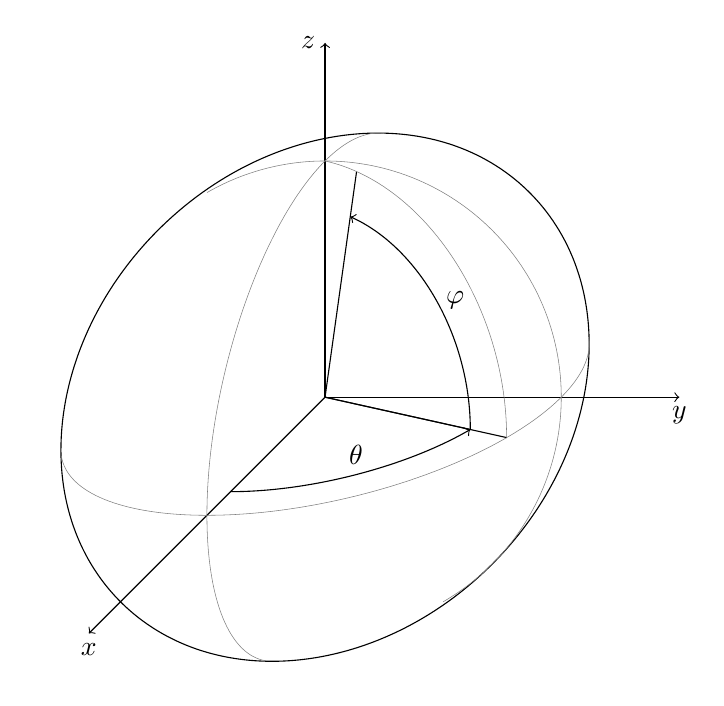
\begin{tikzpicture}[z={(0,1)},y={(-1/2,-1/2)}, scale=3]

\draw[->] (0,0,0)--(1.5,0,0) node[below] {$y$};
\draw[->] (0,0,0)--(0,2,0) node[below] {$x$};
\draw[->] (0,0,0)--(0,0,1.5) node[left] {$z$};

\coordinate (ex) at (.70711,0,-.70711);
\coordinate (ey) at (.57735,-.57735,.57735);
\draw[y=(ey),x=(ex)] (0,0) circle (1);

\draw[gray, very thin] (1,0,0) arc (0:150:1);
\draw[gray, very thin] (1,0,0) arc (0:-30:1);
\draw[gray, very thin, x={(0,0,1)}] (1,0) arc (0:150:1);
\draw[gray, very thin, x={(0,0,1)}] (1,0) arc (0:-30:1);
\draw[gray, very thin, y={(0,0,1)}] (1,0) arc (0:120:1);
\draw[gray, very thin, y={(0,0,1)}] (1,0) arc (0:-60:1);

\draw[->] (0,.8) arc (90:20:.8) node [midway,above] {$\theta$};
\draw (0,0) -- (20:.8);

\begin{scope}[x=(20:1),y={(0,0,1)}]
\draw (0,0)--(1,0);
\draw [->] (.8,0) arc (0:80:.8) node [midway,right] {$\varphi$};
\draw (0,0) -- (80:1);
\draw[gray, very thin] (1,0) arc (0:90:1);
\end{scope}
\end{tikzpicture}
\label{spherefigure}
\caption{Polar coordinate system.}
\end{figure}
and now we calculate the function $f(t,u,\xi) = \norm\xi$ in local coordinates:
\begin{align*}
\tilde f &= \norm{r'(\theta, \varphi) (\dot \theta, \dot \varphi)}\\
&= \norm*{\begin{bmatrix}
-\sin\theta \cos\varphi & -\cos\theta \sin\varphi\\
\cos\theta \cos\varphi & -\sin\theta \sin\varphi\\
0 & \cos\varphi
\end{bmatrix}
\begin{bmatrix}
\dot\theta\\
\dot\varphi
\end{bmatrix}
}\\
&= \sqrt{\cos^2(\varphi) \, \dot\theta^2 + \dot\varphi^2}.
\end{align*}

The Euler-Lagrange equations then become, in local coordinates:
\begin{gather*}
\diffp{\tilde f} \theta - \diff*{\diffp{\tilde f}{\dot \theta}}t = 0 \Leftrightarrow \diff*{\left( \frac{\cos^2(\varphi) \dot \theta}{f} \right)}t = 0,\\
\diffp{\tilde f} \varphi - \diff*{\diffp{\tilde f}{\dot \varphi}}t = 0
\Leftrightarrow
\frac{\cos\varphi \sin\varphi \,\dot \theta^2}{f} = \diff*{\left( \frac{\dot \varphi}{f} \right)}t.
\end{gather*}

To find a solution to these equations, we begin by pointing out that the length of a curve does not depend on the parametrization, as long as it does not double back. Therefore, we may, for simplicity, find a unit-speed parametrization. This simplification is equivalent to requiring that $f = 1$, so the equations become
\[\dot \theta = \frac C {\cos^2(\varphi)}, \quad \ddot \varphi = \cos\varphi \sin\varphi \, \dot \theta^2,\]
and the second equation can be simplified to $\ddot \varphi = C^2 \frac{\sin\varphi}{\cos^3 \varphi}$.

Finally, to simplify matters, let us suppose without loss of generality (by rotation) that the starting point of our curve lies in the equator ($\varphi = 0$), and its initial velocity is $\dot\theta = 1$, $\dot \varphi = 0$. Then, the Euler-Lagrange equations become easy to solve, as $\varphi$ constant equal to 0 is a solution of $\ddot \varphi = C^2 \frac{\sin\varphi}{\cos^3 \varphi}$, and $\dot \theta = C = 1$, and so our curve is just a constant speed rotation about the equator. This (and invariance by change of coordinates) proves that the (unit speed) solutions of the Euler-Lagrange equations are great circle rotations.
\end{example}

Of course, this does not solve the problem of length-minimizing curves in the circle, as we would need to ensure that length-minimizing curves are $C^2$, and solutions of the Euler-Lagrange equations do not necessarily minimize the value of the functional. However, this example has served the purpose of exemplifying the method.

\begin{remark}
This method also works for time-dependent conditions, but it is slightly more complicated, because the spaces that the conditions define are not just manifolds, but rather `time-dependent' manifolds. Unfortunately, I do not know of any relevant bibliography on this matter.
\end{remark}

\subsection{Langrange Multipliers}

When solving problems in calculus of optimization in manifolds, sometimes local parametrizations are very messy business. Indeed, even though the implicit function theorem guarantees that the solutions to independent cartesian equations are manifolds in euclidean space, to parametrize these manifolds explicitly is often messy at best, and impossible at worst. This motivates the study of parametrization-independent methods of optimization. The most well-known of these is the method of Lagrange multipliers, which can be extended to the Calculus of Variations in two ways: it can be applied to problems with integral restriction (e.g. curves of a fixed length), see \cite[\S 12.1]{gelfandfomin}, or it can be applied to problems with pointwise (i.e. holonomic) restrictions, as we will see in this subsection. In section \ref{sec:nonholonomic}, we show a more general version of this principle, which can be applied to nonholonomic constraints, and see also remark \ref{nonholoaregeneral} where we show how integral constraints are really just a particular case of nonholonomic constraints.

The main result of this section is the following:

\begin{theorem}\label{lagrangeholonomic}
Let $u_0$ be a curve that minimizes the functional $I(u) = \int f(t,u,\dot u)$ as $u$ ranges over $C^1$ curves starting at $u_\tstart$, ending at $u_\tend$, and satisfying the $k$ cartesian equations $\phi(t,u(t)) = 0$ for all $t$. Suppose that $u_0$ is $C^2$, that $f$ and $\phi$ are $C^2$ in an open set containing all points of the form $(t,u_0,\dot u_0)$ and $(t,u_0)$ respectively, and that $\diffp \phi u$ has rank $k$ on all points of the form $(t,u_0)$. Then, there exists a continuous function $\lambda \colon \left]t_\tstart, t_\tend\right[ \to \R^k$ such that
\begin{equation}\label{eq:lagrangeholonomic}
\diffp f u - \diff*{\diffp f \xi}t = \lambda(t)^\tr \eval*{\diffp{\phi}{u}}_{t,u_0(t)}.
\end{equation}
\end{theorem}

\begin{remark}
The most common way to ensure the condition on the rank of $\diffp \phi u$ is to request that 0 is a regular value of $\phi$.
\end{remark}

\begin{proof}
The proof of this theorem proceeds locally. We will show that, for all $t$, there exists a neighborhood of $t$ and a function $\lambda$ defined on this neighborhood, satisfying \eqref{eq:lagrangeholonomic}. The theorem follows immediately, as the functions thus defined are unique. Indeed, since $\diffp \phi u$ has linearly independent rows, the equation in $\lambda(t)$ given by \eqref{eq:lagrangeholonomic} has at most one solution for each $t$. The remarkable fact is that these solutions exist for all $t$, and form a continuous function.

To show the theorem locally, we use the inverse function theorem. Given $t_0$, since $\diffp\phi u$ has linearly independent rows, we can without loss of generality (by swapping coordinates if necessary) suppose that the $n \times n$ matrix
\[
A = \begin{bmatrix}
\eval*{\diffp\phi u}_{t_0,u_0(t_0)}\\
\begin{matrix}
0 & I
\end{matrix}
\end{bmatrix}
\]
is invertible. Now, let $\Phi(t,u) = (t, \phi(t,u), u_{k+1}, \dots, u_n)$. It is obvious that
\[\Phi'(t_0, u_0(t_0)) =
\begin{bmatrix}
1 & 0\\
* & A
\end{bmatrix},\]
which is invertible and so we are in the conditions of the inverse function theorem.

To simplify notation, let us define $u^1 = (u_1, \dots, u_k)$ and $u^2 = (u_{k+1}, \dots, u_n)$, so that, for example, $\Phi$ can be written as $\Phi(t,u) = (t, \phi(t,u), u^2)$. Then, by the inverse function theorem, there exist open sets in $\R^{n+1}$, say $U$ and $V$ such that:
\begin{enumerate}
\item $(t_0, u_0(t_0)) \in U$,
\item $\Phi$ is a $C^2$ diffeomorphism $U \to V$, and
\item Without loss of generality, we may assume (making $U$ and $V$ smaller if need be) that $U$ is of the form $\left]t_0-\varepsilon, t_0+\varepsilon\right[ \times U_1$ for some open $U_1$.
\end{enumerate}

Since $(t_0, u_0(t_0)) \in U$ and $\Phi(t_0, u_0(t_0)) \in V$, by continuity there exists a neighborhood of $t_0$, say $B = \left]t_0 - \delta, t_0 + \delta\right[$, such that for all $t$ in this neighborhood we have $(t,u_0(t)) \in U$ and $\Phi(t,u_0(t)) \in V$. Furthermore, suppose that $\delta$ is small enough such that, for all $t \in B$, for all $z \in \R^{n}$ of norm less than some $d$, $\Phi(t,u_0(t)) + (0,0,z) \in V$. To show that such a $\delta$ exists, begin by picking a neighborhood of $\Phi(t_0, u_0(t_0))$ of the form $R \left]t_0-\delta_0, t_0 + \delta_0\right[ \times B_{2d}(0, u_0^2(t_0))$ such that $R$ is contained in $V$. Now pick $\delta < \delta_0$ such that $u_0(t)$ differs less than $d$ from $u_0(t_0)$ for $t$ within $\delta$ of $t_0$. This exists by continuity. Then, for $t \in \left]t_0-\delta, t_0 + \delta\right[$ and $z$ of norm less than $d$, we have that
\[\norm*{(0, u_0^2(t_0)) - \left((0, u_0^2(t)) + (0, z)\right)} \leq \norm{u_0^2(t_0) - u_0^2(t)} + \norm z \leq 2d.\]

This shows that $\Phi(t,u_0(t)) + (0,0,z) \in R \subseteq V$, which allows us to define the variation of $I$ at $u_0$ with respect to some variations contained in $B$. More specifically, let $v : [t_\tstart, t_\tend] \to \R^{n-k}$ be a $C^\infty$ function of support contained in $B$. Then, for $\varepsilon$ small enough (such that $\norm{\varepsilon v} \leq d$), for all $t \in B$ we have $(t, \phi(t,u_0(t)), u_0^2(t) + \varepsilon v(t)) \in V$. Then, we may define $u_\varepsilon$ as
\[
u_\varepsilon(t) =
\begin{cases}
u_0(t), & t \not \in \supp v,\\
\Psi(t, \phi(t,u_0(t)), u_0^2(t) + \varepsilon v(t)), & t \in B,
\end{cases}
\]
where $\Psi$ is defined as follows. Since $\Phi$ is of the form $\Phi(t,u) = (t, \phi(t,u), u^2)$, its inverse must be of the form $\Phi^{-1}(t,w) = (t, \psi(t,w), w^2)$. We set $\Psi(t,w) = (\psi(t,w), w^2)$. In other words, $\Psi = \begin{bmatrix} 0 & I \end{bmatrix} \circ \Phi^{-1}$, i.e. $\Psi$ is the inverse of $\Phi$ with the time component thrown out.

Since both branches of this definition are open, agree on the intersection, and each branch is $C^1$, we conclude that $u_\varepsilon$ is also a $C^1$ path. It is also trivial to see that it satisfies the boundary conditions and that $\phi(t, u_\varepsilon(t)) = 0$. Therefore, we must have
\[I(u_\varepsilon) \geq I(u_0)\]

Now, the standard idea is to take the derivative in $\varepsilon = 0$ and apply Leibniz to get that a certain integral expression is null. However, for our purposes it is useful to first split the integral in two parts:
\[I(u_\varepsilon) = \int_{[t_\tstart,t_\tend] \setminus B} f(t,u_0,\dot u_0) \dl2 t + \int_B f(t,u_\varepsilon, \dot u_\varepsilon) \dl2 t.\]

Now, the first expression is constant in $\varepsilon$, so differentiating and applying Leibniz we get
\[\diff{I(u_\varepsilon)}\varepsilon = \int_B \diffp*{f(t,u_\varepsilon, \dot u_\varepsilon)}\varepsilon \dl2 t.\]

The usual chain rule and integration by parts of the calculus of variation yields\footnote{Here is where we use the assumption that $\phi$ is $C^2$ and that $\Phi$ is a $C^2$ diffeomorphism, because we need that the function $\diffp f \xi$ be $C^1$, and so that $\dot u_\varepsilon$ be $C^1$ in $t$ and $\varepsilon$. To ensure that this is the case, we require the assumption that $\Psi$ is $C^2$, and so that $\Phi$ is a $C^2$ diffeomorphism.}
\[
\diff{I(u_\varepsilon)}\varepsilon = \int_B \diffp f u \diffp{u_\varepsilon}\varepsilon + \diffp f {\xi} \diffp{\dot u}\varepsilon \dl2 t = \int_B \left( \diffp f u + \diff*{\diffp f {\xi}}t \right) \diffp{u}\varepsilon \dl2 t.
\]

Note that in the integration by parts we used the fact that partial derivatives commute, and so
\[\diffp{\dot u_\varepsilon}\varepsilon = \diffp{u_\varepsilon(t)}{\varepsilon,t} = \diffp*{\diffp {u_\varepsilon} \varepsilon}t.\]

The term $\diffp u \varepsilon$ plays the part of the variation in the usual proof of the Euler-Lagrange equations. If $\diffp u \varepsilon$ were arbitrary, we would in fact conclude Euler-Lagrange. However, they are not. Intuitively, they are arbitrary, though tangent to the manifold given by the cartesian equations $\phi = 0$. Therefore, one intuits that the term $\diffp f u + \diff*{\diffp f {\dot u}}t$ is always orthogonal to the manifold, which matches up with the expected conclusion, as we know from vector calculus that the space orthogonal to a manifold defined by cartesian equations is generated by $\nabla_x \phi_1, \dots, \nabla_x \phi_k$..

To proceed with the proof, let us investigate $\eval*{\diffp {u_\varepsilon} \varepsilon}_{\varepsilon = 0}$. This can be computed using the chain rule:
\begin{align*}
\eval*{\diffp {u_\varepsilon} \varepsilon}_0 &= \eval*{\diffp*{\Psi(t, \phi(t,u_0(t)), u_0^2(t) + \varepsilon v(t))} \varepsilon}_0\\
&= \eval*{\begin{bmatrix} 0 & I \end{bmatrix} \diffp*{\Phi^{-1}(t, \phi(t,u_0(t)), u_0^2(t) + \varepsilon v(t))} \varepsilon}_0\\
&= \begin{bmatrix} 0 & I \end{bmatrix} (\Phi^{-1})'(t, \phi(t,u_0(t)), u_0^2(t)) (0, 0, v(t))\\
&= \begin{bmatrix} 0 & I \end{bmatrix} \left(\Phi'(\Phi^{-1}(t, \phi(t,u_0(t)), u_0^2(t)))\right)^{-1} (0,0,v(t))\\
&= \begin{bmatrix} 0 & I \end{bmatrix} \left( \Phi'(t, u_0(t)) \right)^{-1} (0,0,v(t)).
\end{align*}

Therefore, the conclusion is that, for all smooth $v$ defined in $B$,
\[
\int_B \left( \diffp f u + \diff*{\diffp f {\xi}}t \right) \begin{bmatrix} 0 & I \end{bmatrix} \left( \Phi'(t, u_0(t)) \right)^{-1} (0,0,v(t))\dl2 t = 0.
\]

Now, we may apply at once the Fundamental Lemma of the Calculus of Variations, to conclude that the last $n-k$ coordinates of the $(n+1)$-dimensional row-vector
\[\left( \diffp f u + \diff*{\diffp f {\xi}}t \right) \begin{bmatrix} 0 & I \end{bmatrix} \left( \Phi'(t, u_0(t)) \right)^{-1}\]
are null.  In other words, we can write this vector in the form
\[\left( \diffp f u + \diff*{\diffp f {\xi}}t \right) \begin{bmatrix} 0 & I \end{bmatrix} \left( \Phi'(t, u_0(t)) \right)^{-1} = (\ell(t),\lambda(t),0)^\tr,\]
for some $\ell : B \to \R$ and $\lambda : B \to \R^k$. Note that these functions are continuous, as they are a product of continuous functions, and we cannot ensure more regularity under only $C^2$ assumptions because of the $\diff*{\diffp f \xi}t$ term.

To finalize, let us try to solve for $\diffp f u + \diff*{\diffp f {\xi}}t$, which we will temporarily refer to as $T(t)$. Simply put, multiplying by $\Phi'$ and applying matrix block multiplication,
\[\begin{bmatrix}0 & T(t)\end{bmatrix} = (\ell(t), \lambda(t), 0)^\tr \Phi'(t,u_0(t)) =
(\ell(t), \lambda(t), 0)^\tr
\begin{bmatrix}
1 & \begin{matrix} 0 & 0 \end{matrix}\\
* & \diffp\phi u\\
* & \begin{matrix}
0 & I
\end{matrix}
\end{bmatrix}.\]

Therefore, we conclude $T(t) = \lambda(t)^\tr \diffp\phi u$, and so the proof is complete.
\end{proof}

\begin{example}
Let us reproduce example \ref{sphere1}, i.e. to find paths of minimal length on the unit sphere.  In this case,
\begin{gather*}
\phi = x^2 + y^2 + z^2 - 1,\\
f = \sqrt{\dot x^2 + \dot y^2 + \dot z^2}.
\end{gather*}

Our variables are $x(t)$, $y(t)$, $z(t)$ and $\lambda(t)$, and our equations are
\begin{gather*}
\diffp f x - \diff*{\diffp f {\dot x}}t = \lambda(t) \diffp \phi x,\\
\text{(Same for $y$ and $z$)},\\
\phi = 0,
\end{gather*}
and these equations simplify to
\begin{gather*}
- \diff*{\frac{\dot x}f}t = 2 \lambda(t) x,\\
\text{(Same for $y$ and $z$)},\\
x^2 + y^2 + z^2 = 1,
\end{gather*}

As in example \ref{sphere1}, let us make the simplifying assumption of unit speed parametrizations, i.e. $f = 1$. With this simplification, our equations become
\begin{gather*}
\diff*[2]{(x,y,z)}{t} = -2 \lambda(t) (x,y,z),\\
x^2 + y^2 + z^2 = 1.
\end{gather*}

In what follows, let $q = (x,y,z)$. The previous equations state that
\[\ddot q = - 2 \lambda q, \quad \norm{q}^2 = 1.\]

If we can show that $\lambda$ is constant equal to $1/2$, $q$ obeys the Harmonic Oscillator equation, and it is easy to then write out the solutions explicitly as sines and cosines to obtain great circles. Therefore, it suffices to try and solve for $\lambda$. To this effect, we use the following trick. Since we are assuming that $q$ has constant norm, we get that $\braket{\dot q, q} = 0$ by the product rule. Differentiating this expression a second time, we get
\[0 = \diff{\braket{\dot q, q}}t = \braket{\ddot q, q} + \braket{\dot q, \dot q}.\]

Since $\ddot q = - 2 \lambda q$ and we are assuming a unit speed parametrization, this gives
\[0 = - 2 \lambda + 1.\]

Consequently, $\lambda$ is constant equal to $1/2$, and the example is complete.
\end{example}

\section{Nonholonomic Constraints}\label{sec:nonholonomic}

\subsection{Introduction}

In the previous section, we went over problems with holonomic (pointwise) constraints, i.e. optimization problems where the path $u$ to be optimized must satisfy $k$ (independent) cartesian equations of the form $\phi(t,u) = 0$. For a \emph{nonholonomic} problem, the constraints are now differential equations of the form $\phi(t,u,\dot u) = 0$.

Problems with nonholonomic constraints occur often when describing physical systems. The classical example is that of an upright disk rotating without slipping on the $xy$ plane. It is described by four coordinates: the $(x,y)$ coordinates of the disk's center, the angle of the disk about the vertical axis, which we call $\varphi$, and the disk's rotation about its normal axis, which we call $\theta$. See figure \ref{diskfigure}.

\begin{figure}
\centering
\begin{tikzpicture}[z={(0,1)},y={(-1/2,-1/2)}, scale=1.2]

\foreach \x in {1,2,3,4,5}
	\draw[gray, very thin] (\x,0,0) -- (\x,5,0);
\foreach \y in {1,2,3,4}
	\draw[gray, very thin] (0,\y,0) -- (6,\y,0);

\draw[->] (0,0,0)--(6,0,0) node[below] {$y$};
\draw[->] (0,0,0)--(0,5,0) node[below] {$x$};
\draw[->] (0,0,0)--(0,0,4) node[left] {$z$};

\coordinate (circlepos) at (4,3,0);
\coordinate (ev) at (30:1);

\fill[red] (circlepos) circle (0.1);

\begin{scope}[shift=(circlepos),x=(30:1),y={(0,0,1)}]
\draw (0,2) circle (2);
\draw[->] (0,0) -- (2,0);
\draw (0,0) -- (0,2) -- +(-130:2);
\draw[->] (0,0.8) arc (-90:-130:1.2) node[midway,below left] {$\theta$};
\end{scope}

\draw (circlepos) --+(0,1,0);
\draw[->] (circlepos)+(0,1,0) arc (90:30:1) node [midway, below] {$\varphi$};

\node[shift={(-.6,.4)}] at (circlepos) {$(x,y)$};
\end{tikzpicture}
\label{diskfigure}
\caption{The coordinate system for the rolling upright disk.}
\end{figure}

Then, even though all four coordinates can attain any number, they are not independent. If the $\theta$ angle changes a little bit, that induces a change in $x$ and $y$ that depends on $\varphi$. In physics texts, this condition is often described using infinitesimals, as follows
\[\dl x = \cos \varphi \, \dl \theta, \quad \dl y = \sin \varphi \, \dl \theta.\]

For our mathematical purposes, we `divide by $\dl t$' to obtain the ordinary differential equation
\[
\begin{cases}
\dot x = \cos \varphi \, \dot \theta,\\
\dot y = \sin \varphi \, \dot \theta.
\end{cases}
\]

Therefore, if we intend to model the possible paths such a rolling disk might take, they ought to satisfy this differential equation.

In dealing with holonomic constraints, it was essential to assume that the equations of constraint were independent, in the sense that the space-coordinate derivative had full rank. Such an assumption is also necessary here, except that  as we now wish to ensure that a collection of \emph{differential} equations is independent, we consider the derivative in the velocity-coordinate.

\begin{statement}
A problem of optimization with nonholonomic constraints is that in which we intend to minimize the value of the functional $I(u) = \int f(t, u, \dot u) \dl2 t$ under the constraints:
\begin{enumerate}
\item $u$ has prescribed initial and final conditions, i.e. $u(t_\tstart) = u_\tstart$ and $u(t_\tend) = u_\tend$, and
\item $u$ satisfies the equation $\phi(t,u,\dot u) = 0$, where
\[\phi \equiv \phi(t, u, \xi) \colon \R \times \R^n \times \R^n \to \R^k.\]
\end{enumerate}

The $k$ differential equations $\phi = 0$ are said to be \emph{independent} if the $k \times n$ matrix given by $\diffp \phi \xi$ has rank $k$, i.e. has linearly independent rows.
\end{statement}

\begin{remark}\label{pfaffian}
In most applications, $\phi$ is given in the so-called Pfaffian form, i.e.
\[\phi(t,u,\xi) = A(t,u) \xi + b(t,u),\]
for some matrix $A$ and vector $b$. In this case, the requirement of independence of the equations corresponds to requiring that the rows of $A$ are linearly independent.
\end{remark}

\begin{remark}
The definition we have just given is not universal. Indeed, in physics, the term nonholonomic is usually reserved for constraints which \emph{cannot} be made holonomic. So, for example, a constraint of the form $\dl x = \dl y + \dl z$ would not be nonholonomic, because it is equivalent to $x = y + z + C$ for some fixed $C$.

However, in this document the distinction is not useful, and we will use the term nonholonomic for any problem whose constraints are differential equations. Indeed, we consider holonomic problems a subset of nonholonomic problems (see remark \ref{nonholoaregeneral} below.
\end{remark}

\begin{remark}\label{nonholoaregeneral}
A wide class of problems can be seen as nonholonomic. For example, any holonomic problem can be seen in this framework.

Consider a holonomic problem with restriction $\phi(t,u) = 0$. The obvious way to transform it into a nonholonomic problem would be to simply write $\wtphi(t,u,\xi) = \phi(t,u)$. However, $\wtphi$ does not satisfy the independence requirement for nonholonomic problems, which means that our methods will not be applicable. Instead, a better way to turn a holonomic problem into a nonholonomic one would be to note that $\phi(t,u)$ is constant, and so, differentiating in time, $\diffp \phi u \dot u + \diffp \phi t = 0$. This can be seen as a nonholonomic constraint in Pfaffian form, and it is easy to see that independence of the holonomic equations $\phi = 0$ is equivalent to independence of the nonholonomic equations $\psi = 0$, where $\psi(t,u,\xi) = \eval*{\diffp \phi u}_{t,u} \xi + \eval*{\diffp \phi t}_{t,u}$ (see remark \ref{pfaffian}).

Another class of problems that can be seen in nonholonomic form is problems with functional constraints. That is, suppose we wish to consider paths $u$ satisfying $\int g(t,u,\dot u) \dl t = c$. Such a constraint can be written as a differential equation by adding an auxiliary quantity, which we call $j(t)$, which represents $\int_\tstart^t g$. Then, we add the constraints
\[j(t_\tstart) = 0, \quad j(t_\tend) = c, \quad \diff j t = g(t,u,\dot u).\]
\end{remark}

\subsection{Valid Displacements}\label{validdisplacements}

The strategy used to prove the basic form of the Euler-Lagrange equations, which consists of adding a perturbation to a path $u_0$ which is assumed to minimize $I(u)$, requires vector space structure, which is lost when we restrict our paths to those satisfying nonlinear conditions. In the holonomic case, this problem was recoverable by using the inverse/implicit function theorem to locally `distort the space into $\R^n$'.

Unfortunately, such strategies fall completely flat when passing to the nonholonomic case. Because of the differential nature of the restrictions, small perturbations will propagate from the place of perturbation to the end of the path. The easiest way to see this is to imagine a problem in which the constraint is given by $\norm{\dot u} = 1$. Then, a straight line cannot possibly be perturbed without changing the initial or final location. This means that we necessarily have to give up on the strategy of considering small admissible perturbations of a minimal path.

Therefore, our strategy will be to consider perturbations that keep only the start of the path fixed. We will concern ourselves with the end later on. But even lifting this restriction, it is not obvious that \emph{any} nontrivial perturbation exists, or how to construct it. It is here that the hypothesis of independence of the differential equations comes into play, because it allows is to apply a kind of implicit/inverse function theorem, which we will now state. The proof of this theorem is left to appendix \ref{buffift}. For an alternative proof, we direct the reader to \cite[\S 3]{blissmayer}.

\begin{restatable}{theorem}{buffift}\label{thm:buffift}
Let $u \colon [t_\tstart,t_\tend] \to \R^n$ be a $C^p$ curve, for $p \in \N_0$, $\Omega$ an open subset of $X = \R \times \R^n \times \R^n$ such that $(t,u(t),\dot u(t)) \in \Omega$ for all $t$, and $\phi \equiv \phi(t,u,\xi)$ a $C^{p+1}$ function $\phi \colon \Omega \to \R^k$.

Suppose that for all $t$ the matrix $\diffp\phi\xi$ has rank $k$. Then there exist open subsets of $X$, say $U$ and $V$, and a function $\wtphi \colon U \to \R^n$, such that
\begin{itemize}
\item $U$ contains all points of the form $(t,u(t),\dot u(t))$,
\item $U$ is contained in $\Omega$,
\item The first $k$ coordinates of $\wtphi$ agree with $\phi$
\item The function given by
\begin{align*}
\Phi \colon U &\to V\\
(t,u,\xi) &\mapsto (t,u,\wtphi(t,u,\xi))
\end{align*}
is a $C^p$ diffeomorphism.
\end{itemize}
\end{restatable}

We will now use this theorem to build our perturbations of a path. Indeed, given a path $u_0$, construct the $U$, $V$, and $\Phi$ given above. Let the inverse of $\Phi$ be denoted $(t,u,\xi) \mapsto (t,u,\psi(t,u,\xi))$.

We can use $\psi$ to build a valid displacement of $u$ as follows. We wish to find a perturbation of $u$, let's say $\tilde u$, such that $\phi(t,u,\dot u) = 0$. Therefore, $\wtphi(t,u,\dot u)$ is of the form $(0,w(t))$ for some $v$. This can be solved for $\dot u$, and we get the differential equation
\[\dot u(t) = \psi(t,u(t),w(t)).\]

We can now use ODE theory to guarantee that this has a solution for $w$ `close enough to $w_0$', for `$w_0$ corresponding to the path $u_0$'.

\begin{theorem}\label{thm:perturbation}
Let $p \in \N^+$.\footnote{We will only use the case $p = 1$.} Let $u$ be a $C^{p+1}$ path satisfying $\phi(t,u,\dot u) = 0$ for $\phi$ a $C^p$ function such that $\diffp \phi \xi$ has linearly independent rows. Extend $\phi$ to $\wtphi$ (in a $C^p$ way) using the methods of theorem \ref{thm:buffift}. Let $\wtphi(t,u,\dot u) = (0, w(t))$. Then, given a curve $v : [t_\tstart, t_\tend] \to \R^{n-k}$ of class $C^p$ in this interval, for real numbers $b$ close enough to zero the following ODE has a unique solution with $(t,u,\dot u) \in U$:
\[
\begin{cases}
\wtphi(t, u, \dot u) = (0, w(t) + b\,v(t)),\\
u(t_\tstart) = u_\tstart.
\end{cases}
\]

For $b$ small enough that this exists, we refer to this solution as $u_b^v(t)$, or $u_b$ if $v$ is implied.

The resulting function of two parameters ($b$ and $t$) is $C^p$.
\end{theorem}

\begin{proof}
We begin by applying theorem \ref{thm:buffift} to $\phi$, to obtain the $U$, $V$ and $\Phi$ therein described. Let
\[\Phi^{-1}(t,u,\xi) = (t,u,\psi(t,u,\xi)).\]

Note that all points of the form $(t,u(t),0,w(t))$ are in $V$, for $t \in [t_\tstart, t_\tend]$. The set of these points form a compact set, and it is known from metric space theory that there exists a $\delta > 0$ such that for all $z$ with $\norm z < \delta$ we have $(t,u,0,w) + z \in V$ for all $t$. Consequently, if $b < \delta / \max \norm v$, $(t,u,0,w+bv) \in V$, and so\footnote{It is subtle, but this `if and only if' is where we use the hypothesis that $(t,u,\dot u) \in U$.}
\[\wtphi(t, u, \dot u) = (0, w(t) + b\,v(t)) \text{ iff } \dot u(t) = \psi(t,u(t),w(t) + b\,v(t)).\]

Therefore, (for small enough $b$) our ODE is of the form
\[
\begin{cases}
\dot u(t) = F(t,u(t),b),\\
u(t_\tstart) = u_\tstart,
\end{cases}
\]
to which elementary ODE theory is applicable. Note that since $\psi$, $w$, and $v$ are $C^p$, $F$ is also $C^p$. In particular, it is $C^1$, and so (see \cite[p.74]{perko}) the solution exists and is unique for small enough $t$. Moreover, it is known to exist in $[t_\tstart, t_\tend]$ for $b = 0$ (it is $u_0$ in this case), and consequently (see \cite[thm.2,~p.84]{perko}) the solution exists and is unique for $t \in [t_\tstart,t_\tend]$, for $b$ close enough to 0.

To show differentiability in these two variables, the cited reference proves only the case $p = 1$. However, the methods therein found can be used to prove inductively for all $p \in \N^+$ that if $F$ is $C^p$ then $u$ is also $C^p$ in time and the parameters.
\end{proof}

\begin{remark}\label{rmk:perturbation}
Though the above proof was stated for only one parameter $b$, it could easily be stated and extended for several parameters and $v$'s. In other words, we could have considered the ODE
\[
\begin{cases}
\wtphi(t, u, \dot u) = (0, w(t) + b_1\,v_1(t) + \dots + b_q v_q(t)),\\
u(t_\tstart) = u_\tstart.
\end{cases}
\]

The same result and notation applies, except that we collect the functions $v_i$ in a $(n-k) \times q$ matrix we call $V(t)$, and the scalars $b_i$ form a vector we call $\vecb$. This will be crucial in section \ref{sec:multrule}, which contains the main result of this document: the multiplier rule.
\end{remark}

\subsection{First Variation}\label{sec:firstvar}

Consider a one-parameter family of arcs of the form $u_b^v(t)$, constructed as described above. We will abbreviate this to $u_b(t)$. We will now investigate the behavior of $I(u_b)$ around zero: more precisely, we will study $\diff{I(u_b)}b[0]$, i.e. the first variation of $I$ along this family.

Recall that $I(u_b)$ is defined as $\int f(t, u_b(t), \dot u_b(t)) \dl1 t$, and since this is integration over a compact interval of a $C^1$ function in both its variables (assuming $f$ is $C^1$ and $u_b(t)$ is $C^2$ jointly in both variables) Leibniz' rule is applicable and so
\[\diff{I(u_b)}b = \int_\tstart^\tend \diffp*{f(t, u_b, \dot u_b)}b \dl1 t =\int_\tstart^\tend \diffp f u \diffp{u_b}b + \diffp f \xi \diffp{\dot u_b}b \dl1 t.\]

If we now assume that $f$ is $C^2$, the usual integration by parts of the calculus of variations can be performed. In doing so, we are implicitly using the fact that, since $u$ is $C^2$ in $b$ and $t$, the order of derivatives is irrelevant, and thus $\diffp{\dot u_b}b = \diffp{u_b(t)}{t,b}$. We conclude
\[\diff I b = \int_\tstart^\tend \left( \diffp f u - \diff*{\diffp f \xi}t \right) \diffp{u_b}b \dl1 t + \bracket*{ \diffp f \xi \diffp{u_b}b }_\tstart^\tend.\]

Finally, note that we are keeping the first end of $u$ fixed, so that $u_b(t_\tstart)$ is constant and so $\eval*{\diffp{u_b}b}_\tstart = 0$. Therefore, the bracket term can be simplified, yielding
\begin{equation}\label{firstvar1}
\diff I b = \int_\tstart^\tend \left( \diffp f u - \diff*{\diffp f \xi}t \right) \diffp{u_b}b \dl1 t + \eval*{\diffp f \xi}_\tend \eval*{\diffp{u_b}b}_\tend.
\end{equation}

In order to avoid writing a burdensome amount of terms, we now introduce a notation for the `Euler-Lagrange derivative'. Let $\Theta$ be the differential operator given by
\[\Theta(f) := \diffp f u - \diff*{\diffp f \xi}t.\]

With this notation, \eqref{firstvar1} can be written
\begin{equation}\label{firstvar2}
\diff I b = \int_\tstart^\tend \Theta(f) \diffp{u_b}b \dl1 t + \eval*{\diffp f \xi}_\tend \eval*{\diffp{u_b}b}_\tend.
\end{equation}

There exists a trick that will later be used to get rid of the non-integral terms, which we now describe. Recall that $u_b$ satisfies the differential equation
\[\wtphi(t,u_b(t),\dot u_b(t)) = (0, w(t) + b\,v(t)),\]
where $\wtphi(t,u_0,\dot u_0) = (0,w(t))$. This actually consists of $n$ differential equations, which can be added together. Indeed, if $\mu(t) = (\mu_1(t), \mu_2(t))$ is a regular enough time-dependent $n$-vector,
\[\mu \cdot \wtphi(t, u, \dot u) = \mu_2 \cdot w + b \, \mu_2 \cdot v.\]

Taking the partial derivative in $b$, we obtain
\[\mu \cdot \diffp{\wtphi}u \diffp u b + \mu \cdot \diffp{\wtphi}\xi \diffp{\dot u}b = \mu_2 \cdot v,\]
which can be rewritten in terms of $\Theta$ as
\[\Theta(\mu \cdot \wtphi) \diffp u b = \mu_2 \cdot v - \diff*{\left(\diffp{(\mu \cdot \wtphi)}\xi \diffp u b \right)}t.\]

Integrating, this yields
\[\int_\tstart^\tend \Theta(\mu \cdot \wtphi) \diffp u b \dl1 t = \int_\tstart^\tend \mu_2 \cdot v \dl2 t - \bracket*{\diffp{(\mu \cdot \wtphi)}\xi \diffp u b}_\tstart^\tend.\]

Using the same trick as before, the bracket can be simplified to get
\[\int_\tstart^\tend \Theta(\mu \cdot \wtphi) \diffp u b \dl1 t = \int_\tstart^\tend \mu_2 \cdot v \dl2 t - \mu(t_\tend) \cdot \eval*{\diffp{\wtphi}\xi}_\tend \eval*{\diffp u b}_\tend.\]

Adding and subtracting this expression to a multiple of $\diff I b$, using \eqref{firstvar2} we get
\begin{multline}\label{firstvar3}
\ell_0 \diff I b = \int_\tstart^\tend \Theta(\ell_0 f + \mu \cdot \wtphi) \diffp{u_b}b \dl1 t - \int_\tstart^\tend \mu_2 \cdot v \dl2 t\\
+ \left(\ell_0 \eval*{\diffp{f} \xi}_\tend + \mu(t_\tend)^\tr \eval*{\diffp\wtphi\xi}_\tend \right) \eval*{\diffp{u_b}b}_\tend.
\end{multline}

Even though this expression looks more complex than \eqref{firstvar2}, it has a large degree of freedom to exploit: $\mu$ has been left arbitrary (as long as it is $C^1$ so that the $\Theta$ term exists). For example, we could cross out the non-integral term by choosing an appropriate value for $\mu(t_\tend)$. We will not do so yet, however, because an even more appropriate choice will present itself in due time. The mysterious $\ell_0$ coefficient appears for technical reasons, and is necessary in a proof. If the reader is mystified by its presence, he or she may ignore it for now.

\subsection{The Multiplier Rule}\label{sec:multrule}

In this section, we will finally prove the necessary condition for a minimum that we have been building up to: the Lagrange Multipler Rule.

Suppose that that $u_0$ is a minimum of the functional $I$ over the class of paths such that $u(t_\tstart) = u_\tstart$, $u(t_\tend) = u_\tend$ and $\phi(t,u,\dot u) = 0$, under the hypothesis that $f$ is $C^2$, $u_0$ is $C^2$ and $\phi$ is $C^3$ and that $\diffp \phi \xi$ has full rank over the path $u_0$.

We might be tempted to apply the formula \eqref{firstvar2} or \eqref{firstvar3} for $\diff I b$ and claim that $\diff I b = 0$ for all $v$, since $u_0$ minimizes the value of $I$. However, that is neglecting the requirement that $u(t_\tend) = u_\tend$: since the variations we have created break this requirement, $I(u_b)$ has no obligation to be minimal at $b = 0$. One could consider restricting themselves to variations $v$ that guarantee the boundary conditions, but such $v$ might not even exist: consider the example where $u_0$ is a straight line and $\phi(t,u,\xi) = \norm \xi$.

To get around this, consider an arbitrary collection $v_1, \dots, v_{n+1}$ of smooth functions $[t_\tstart, t_\tend] \to \R^{n-k}$, which we collect into the matrix $V(t)$. We can see $I$ as function in $n+1$-variables, given by the vector $\vecb$ (see remark \ref{rmk:perturbation}). Furthermore, we can see $u(t_\tend)$ as a function of $\vecb$ as well, and so we can consider the function (with $n+1$ variables and values in $\R^{n+1}$) given by
\begin{equation}\label{vecbfunc}
\vecb \mapsto (I(u_\vecb^V), u_\vecb(t_\tend)).
\end{equation}

This function is $C^1$ in a neighborhood of the origin. To see why, first note that theorem \ref{thm:perturbation} guarantees that $u_\vecb(t)$ is $C^2$ as a function of both parameters, and so in particular is $C^1$ if we fix $t = t_\tend$. This shows that the last $n$ coordinates of \eqref{vecbfunc} are $C^1$. It now suffices to show that $I(u_\vecb^V)$ is $C^1$. To do so, note that $f$ is $C^1$ in its three arguments: $t$, $u_\vecb^V(t)$ and $\dot u_\vecb^V(t)$. Furthermore, since all its arguments are $C^1$ in $t$ and $\vecb$ (here we use that $\phi$ is $C^3$ to show that $u$ is $C^2$ in $t$ and $\vecb$ and so $\dot u$ is $C^1$ in $\vecb$), we get that so is the composite, and Leibniz' theorem guarantees that an integral in $t$ of a $C^1$ function in $t$ and $\vecb$ is $C^1$ in $\vecb$.

Since \eqref{vecbfunc} is $C^1$ from $n+1$-dimensional space to $n+1$-dimensional space, we are in conditions of applying the inverse function theorem. We conclude that if the jacobian of \eqref{vecbfunc} at $\vecb = 0$ were invertible, \eqref{vecbfunc} would be a diffeomorphism in a neighborhood of the origin. But this contradicts the assumption that $u_0$ is a minimum of $I$, for in this case we could find $\vecb$ such that $u_\vecb(t_\tend) = u_\tend$, and $I(u_\vecb^V)$ is slightly smaller than $I(u_0)$. In other words, under the assumption that $u$ is a minimum of $I$, the following matrix has linearly dependent columns: (evaluated at $\vecb = 0$)
\[
\begin{bmatrix}
\displaystyle \diffp*{I(u_\vecb^V)}{b_1} & \dots & \displaystyle \diffp*{I(u_\vecb^V)}{b_{n+1}}\\[1em]
\displaystyle \diffp*{u_\vecb^V(t_\tend)}{b_1} & \dots &\displaystyle \diffp*{u_\vecb^V(t_\tend)}{b_{n+1}}
\end{bmatrix}.
\]

Note that, at $\vecb = 0$, these columns can be simplified:
\[
\begin{bmatrix}
\displaystyle \diff*{I(u_b^{v_1})}{b} & \dots & \displaystyle \diff*{I(u_b^{v_{n+1}})}{b}\\[1em]
\displaystyle \diff*{u_b^{v_1}(t_\tend)}{b} & \dots & \displaystyle \diff*{u_b^{v_{n+1}}(t_\tend)}{b}
\end{bmatrix}.
\]

Since this holds for arbitrary collections $v_1, \dots, v_{n+1}$, we can actually conclude a surprisingly strong result. Let $q$ be the maximal possible number of $v_1, \dots, v_q$ such that the following matrix has linearly independent columns
\[
A =
\begin{bmatrix}
\displaystyle \diff*{I(u_b^{v_1})}{b} & \dots & \displaystyle \diff*{I(u_b^{v_{q}})}{b}\\[1em]
\displaystyle \diff*{u_b^{v_1}(t_\tend)}{b} & \dots & \displaystyle \diff*{u_b^{v_{q}}(t_\tend)}{b}
\end{bmatrix}.
\]

By the above, $q < n+1$. Therefore, for any $v$, the vector $(\diff*{I(u_b^v)}{b}, \diff*{u_b^v(t_\tend)}{b})$ is a linear combination of the columns of $A$, i.e. of the form $Aw$ for some $w \in \R^{n+1}$.

Since the matrix $A$ has more rows than columns, there exists a row-matrix, say $E = \begin{bmatrix} \ell_0 & e \end{bmatrix} = \begin{bmatrix} \ell_0 & e_1 & \dots & e_n\end{bmatrix}$, such that $E A = 0$. By the previous paragraph, we conclude that \emph{for this specific collection of scalars}(!), for any smooth $v$ we have
\begin{equation}\label{premultiplier}
\ell_0 \diff*{I(u_b^v)}{b} + e \diff*{u_b^v(t_\tend)}{b} = 0.
\end{equation}

We can now rewrite the variation in $I$ using \eqref{firstvar3} to get
\begin{multline*}
\ell_0 \diff I b = \int_\tstart^\tend \Theta(\ell_0 f + \mu \cdot \wtphi) \diffp{u_b}b \dl1 t - \int_\tstart^\tend \mu_2 \cdot v \dl2 t\\
+ \left(\ell_0 \eval*{\diffp{f} \xi}_\tend + \mu(t_\tend)^\tr \eval*{\diffp\wtphi\xi}_\tend \right) \eval*{\diffp{u_b}b}_\tend,
\end{multline*}
where, as the reader will recall, $\mu$ has been left as an arbitrary $C^1$ function. Substituting in \eqref{premultiplier}, we obtain
\begin{multline}\label{bigequation}
\int_\tstart^\tend \Theta(\ell_0 f + \mu \cdot \wtphi) \diffp{u_b}b \dl1 t - \int_\tstart^\tend \mu_2 \cdot v \dl2 t\\
+ \left(\ell_0 \eval*{\diffp{f} \xi}_\tend + \mu(t_\tend)^\tr \eval*{\diffp\wtphi\xi}_\tend + e\right) \eval*{\diffp{u_b}b}_\tend = 0, \text{ for all regular $v$.}
\end{multline}

Even though this looks like a very complicated expression, this is where the arbitrariness of $\mu$ comes into play. For instance, we can now pick $\mu(t_\tend)$ to make
\[\ell_0 \eval*{\diffp{f} \xi}_\tend + \mu(t_\tend)^\tr \eval*{\diffp\wtphi\xi}_\tend + e = 0.\]

This is possible because $\diffp\wtphi\xi$ is invertible. Note that this choice is independent of $v$.

As a further simplification, we may wish to ensure that $\Theta(\ell_0 f + \mu \cdot \wtphi)$. Expanding the expression, we get the following linear ODE:
\begin{equation}\label{thetaode}
\ell_0 \diffp f u + \mu^\tr \diffp \wtphi u = \ell_0 \diff*{\diffp f \xi}t + \mu^\tr \diff*{\diffp \wtphi \xi}t + \dot \mu^\tr \diffp \wtphi \xi,
\end{equation}
where all partial derivatives are evaluated on the vector $(t,u_0(t),\dot u_0(t))$. Since $\diffp \wtphi \xi$ is invertible, this can be rewritten as a linear ODE of the form
\begin{equation}\label{thetaode2}
\dot \mu(t) = A(t) \mu(t) + B(t).
\end{equation}

Classical ODE theory guarantees that \eqref{thetaode2} has unique solution for all time, given initial conditions (see \cite[pp.~60,61]{perko}). Therefore, we may construct a concrete $\mu$ as the unique solution to
\begin{equation}\label{thetaode3}
\begin{cases}
\Theta(\eval*{\ell_0 f}_{t,u_0(t),\dot u_0(t)} + \mu(t) \cdot \wtphi(t,u_0(t),\dot u_0(t)),\\
\ell_0 \eval*{\diffp{f} \xi}_\tend + \mu(t_\tend)^\tr \eval*{\diffp\wtphi\xi}_\tend + e = 0.
\end{cases}
\end{equation}

For this particular $\mu$, \eqref{bigequation} simplifies to
\[\int_\tstart^\tend \mu_2 \cdot v \dl2 t = 0 \text{ for all regular $v$.}\]

We may now apply the FLCV to get that the last $k$ coordinates of $\mu$ are null, and so
\[\Theta(\ell_0 f + \mu_1 \cdot \phi) = 0\]

This is good, because this result does not depend on any arbitrary choices, such as the extension of $\phi$ to $\wtphi$. Therefore, we have the first version of the Lagrange multiplier rule:

\begin{theorem}
Let $u_0$ be a $C^2$ minimum of the optimization problem
\[\min I(u) = \int f,\]
where $f$ is $C^2$ and $u$ varies over $C^1$ paths satisfying $u(t_\tstart) = u_\tstart$, $u(t_\tend) = u_\tend$, and the $k$ differential equations given by
\[\phi(t,u(t),\dot u(t)) = 0,\]
where $\phi$ is a $C^3$ function with $k$ coordinates. Suppose that these $k$ equations are independent differential equations, in the sense that $\diffp \phi \xi$ has rank $k$ over the whole path. Then, there exists a constant $\ell_0$ and $k$ $C^1$ functions, say $\lambda_1, \dots, \lambda_k$, such that the following differential equation is satisfied in $[t_\tstart, t_\tend]$.
\begin{equation}\label{multipliers}
\ell_0 \diffp f u + \lambda \cdot \diffp \phi u = \diff*{\left(\ell_0 \diffp f \xi + \lambda^\tr \diffp \phi \xi\right)}t.
\end{equation}

Furthermore, it is not the case that $\ell_0$, $\lambda_1$, \dots, $\lambda_k$ are all null.
\end{theorem}

\begin{remark}
The condition that not all be null is essential to stop the theorem from becoming a triviality: otherwise, the trivial solution would always be possible.

To show that not all are null, suppose that $\ell_0$ is null. Then, by \eqref{thetaode3} $\lambda$ satisfies
\[\lambda(t_\tend)^\tr \eval*{\diffp\wtphi\xi}_\tend + e = 0.\]

Since by hypothesis the row-matrix $E = \begin{bmatrix}\ell_0 & e\end{bmatrix}$ is non-null, and we are assuming that $\ell_0$ is null, and so $e$ cannot be, and therefore $\lambda(t_\tend)$ cannot be as well. By continuity, we conclude that $\lambda$ cannot be the null function.
\end{remark}

\begin{remark}
As it ought to, the problem posed by \eqref{multipliers} has as many equations as it has variables, if we consider the solution of the problem to be the process of finding the $u_0$. Indeed, we have $n+k$ functions to find:
\[u_1, \dots, u_n, \lambda_1, \dots, \lambda_k,\]
and $k+n$ equations: $k$ are given by the condition $\phi(t,u,\dot u) = 0$, and $n$ are given by \eqref{multipliers}. It is by solving this problem in $n+k$ variables and equations that one usually solves this kind of variational problems.
\end{remark}

\subsection{Normality and Abnormality}

Consider the parameter $\ell_0$ in the Lagrange multiplier equations, \eqref{multiplers}. There exist two possible cases:
\begin{itemize}
\item If $\ell_0 \neq 0$, the whole equation can be divided by $\ell_0$, yielding solutions to the equation
\begin{equation}\label{multipliers:normal}
\diffp f u + \lambda \cdot \diffp \phi u = \diff*{\left(\diffp f \xi + \lambda \cdot \diffp \phi \xi\right)}t.
\end{equation}

This is the so-called \emph{normal case};

\item If $\ell_0 = 0$, we obtain a \emph{nontrivial} solution to the equation
\begin{equation}\label{multipliers:abnormal}
\lambda \cdot \diffp \phi u = \diff*{\left(\lambda \cdot \diffp \phi \xi\right)}t.
\end{equation}

This is the so-called \emph{abnormal} case.
\end{itemize}

The solutions to the Lagrange multiplier equation can be divided into two types: normal solutions, wherein $\ell_0 \neq 0$, and abnormal solutions, where $\ell_0 = 0$.

An analogy can be made between the distinction normal/abnormal solutions and the distinction interior/border of a manifold. In some sense, as the name would indicate, abnormal solutions are `undesired', or uncommon. In fact, note that the existence (or not) of abnormal solutions \emph{does not depend on the functional being considered}, but only on the constraints placed on the paths! This is by analogy to optimization in calculus, where, besides checking critical points of the function to be optimized, one must usually also check the border of the space for extrema. According to Brunt \cite[p.~129]{brunt}, the usual approach to variational problems with nonholonomic constraints is to work under the assumption that the problem is normal, i.e. that there are no abnormal extrema, and only afterwards study the abnormal solutions and compare them to the normal critical points found.

Geometrically, abnormal solutions correspond to solutions that cannot be perturbed. For example, in a constant-speed nonholonomic problem, a straight line cannot be perturbed while preserving the boundary conditions, while a non-straight line can be slightly perturbed. This particular case can easily be verified:

\begin{theorem}\label{abnormalline}
Let $\phi(t,u,\xi) = \xi^2 - 1$. Then, $u$ is an abnormal solution to the Euler-Lagrange equations if and only if it is a straight line.
\end{theorem}

\begin{proof}
The equation to be solved is given by \eqref{multipliers:abnormal}, which in this case reduces to
\[0 = \diff{(2 \lambda \dot u)}t,\]
i.e. the vector $\lambda \dot u$ is constant. Furthermore, we are under the constraint $\norm{\dot u} = 1$, so taking the norm of $\lambda \dot u$ we obtain that $\lambda$ is constant, and by nontriviality of the solution must be a constant different from zero. Therefore, $\dot u$ must be constant, and so $u$ is a (speed 1) straight line.
\end{proof}

\subsection{Example of application}

Let us apply the method of Lagrange multipliers to Dido's problem, of finding a curve of fixed length $L > 2$, starting at $(-1,0)$ and ending at $(1,0)$, that encompasses the most area between it and the $x$ axis. To do so, we encode the problem as a variational problem with nonholonomic constraints.

In order to consider curves of fixed length $L$, instead of considering an integral constraint on the paths, we will consider paths of unit speed defined on $[0,L]$. That is, if we let $u = (x,y)$, our restrictions are given by
\begin{equation}\label{initcond}
x(0) = -1,\; x(L) = 1, \quad y(0) = y(L) = 0, \quad \dot x^2 + \dot y^2 - 1 = 0.
\end{equation}

To measure the area encompassed by the curve\footnote{The usual remark about the equivalence of maximization and minimization problems applies.} $u = (x,y)$, the usual trick is to apply Green's formula on the integral $\int_\Omega 1 \dl1 x \dl1 y$ to get a formula for the area such as
\[I(u) = - \int_0^L x \dot y \dl2 t.\]

Let us now find the Euler-Lagrange equations. By theorem \ref{abnormalline}, the abnormal solutions to the Euler-Lagrange equations are straight lines, and straight lines cannot satisfy the boundary conditions as the start and end points are too close together, at a distance of $2 < L$. Therefore, we need only consider the Euler-Lagrange equations for the normal case, which are
\[
\begin{cases}
\displaystyle \diffp f x + \lambda \diffp \phi x = \diff*{\left(\diffp f {\dot x} + \lambda \diffp \phi {\dot x}\right)}t,\\[0.7em]
\displaystyle \diffp f y + \lambda \diffp \phi y = \diff*{\left( \diffp f {\dot y} + \lambda \diffp \phi {\dot y}\right)}t,\\
\dot x^2 + \dot y^2 = 1,
\end{cases}
\]
where $\lambda$ is a $C^1$ real function, and $u$ satisfies \eqref{initcond}. Expanding the partial derivatives,
\begin{equation}\label{dido1}
\begin{cases}
\dot y  = 2 \dot \lambda \dot x + 2 \lambda \ddot x,\\
0 = \dot x + 2 \dot \lambda \dot y + 2 \lambda \ddot y,\\
\dot x^2 + \dot y^2 = 1.
\end{cases}
\end{equation}

To solve these equations, note that from the restriction $\dot x^2 + \dot y^2 = 1$ we conclude
\[2\lambda \ddot x \dot x + 2 \lambda \ddot y \dot y = 0.\]

Therefore, adding appropriate multiples of the other two equations, we obtain
\[\cancel{\dot y \dot x} = 2 \dot \lambda \dot x^2 + \cancel{\dot x \dot y} + 2 \dot \lambda \dot y^2,\]
and using $\dot x^2 + \dot y^2 = 1$ we get
\[\dot \lambda = 0.\]

Consequently, $\lambda$ is a constant, and \eqref{dido1} reduces to
\begin{equation}\label{dido2}
\begin{cases}
\dot y  = 2 \lambda \ddot x,\\
\dot x = - 2 \lambda \ddot y,\\
\dot x^2 + \dot y^2 = 1.
\end{cases}
\end{equation}

Consequently, $\dot x = - 2 \lambda \ddot y = -4 \lambda^2 \dot{\ddot x}$, and so $\dot x$ is of the form
\[\dot x = A \sin(2 \lambda t) + B \cos(2 \lambda t).\]

If $\lambda = 0$, $x$ would be a constant and so $\ddot x = 0$, implying $\dot y = 0$ and so $(x,y)$ is constant, contradicting the hypothesis of unit speed. Therefore, $\lambda \neq 0$ and so we can integrate $\dot x$ to get
\[x = A' \sin(2 \lambda t) + B' \cos(2 \lambda t) + C,\]
for $A' = \frac1{2 \lambda} B$ and $B' = -\frac1{2\lambda} A$. Integrating $\dot y = 2 \lambda \ddot x$, we get
\[y = A' \cos(2 \lambda t) - B' \sin(2 \lambda t) + C'.\]

We conclude that the curve $(x,y)$ describes a circle around the point $(C, C')$, and so the (multiple) solutions to the Euler-Lagrange equations are unit speed circle sections starting at $(-1,0)$ and ending at $(1,0)$. Further investigation would be necessary to find expressions for these circles and to discover which of them is the best candidate for a maximum.

\subsection{Further reading}

As mentioned in the introduction, this proof is, for the most part, a particularization of the proof found in Bliss \cite[pp.~187-202]{bliss}. We direct the interested reader there, as the theorem is stated and proved in much, much greater generality: the paths considered are sectionally $C^1$, the endpoints of the curves are not fixed but rather obey some set of equations (imagine a chain with endpoints on a rail), $t_\tstart$ and $t_\tend$ are likewise not fixed, and the functional to be optimized might have a term depending on the endpoints. It is reasonably well-written, though in a terse style which, when combined with unusual notational conventions (e.g. the Euler-Lagrange equations are written in integral form) might leave a first-time reader perplexed. I certainly was.

The section on normality and abnormality was loosely based on Brunt \cite[pp.~128,129]{brunt}, which also has a discussion of the (non)applicability of the Lagrange multiplier method to nonholonomic problems in mechanics, as well as further bibliographic references.

\begin{appendices}

\section{An implicit function-like theorem}\label{buffift}

In this appendix, we prove the following auxiliary result, which was used in section \ref{validdisplacements}

\buffift*

The kernel of the proof is the following lemma:

\begin{lemma}\label{matrixlemma}
Let $A(t)$ be a variable $k \times n$ matrix, for $t \in [t_\tstart, t_\tend]$. Suppose that $A$ is a $C^p$ function for some $p \in \N_0$. Then, it is possible to add $n-k$ (variable) rows to $A$, yielding a function $\tilde A(t)$, such that $\tilde A$ is $C^p$ and invertible for all $t$.
\end{lemma}

\begin{proof}
To prove this lemma, we will actually prove something stronger yet. We will show that if $k < n$ then there exists $v(t)$, different from zero, defined on $[t_\tstart, t_\tend]$ such that $v$ is orthogonal to all rows of $A$. Such a $v$ can clearly be appended as a row to $A$, creating a $(k+1) \times n$ matrix of rank $k+1$, and repeating the process $n-k$ times we obtain the desired $\tilde A$.

The main trick in this proof is that, locally, such a $v$ is determined uniquely by $n-k$ well-chosen coordinates. Indeed, we wish to solve the equation $A v = 0$. We know from linear algebra that there exists a $k \times k$ invertible minor of $A$ (which corresponds to the pivots in gaussian elimination). Without loss of generality we can suppose that, for some fixed $t_1$, this minor is the leftmost, i.e. given $t_1$ we can by reordering of coordinates assume that $A(t) = \begin{bmatrix} A_1(t) & A_2(t) \end{bmatrix}$, with $A_1(t_1)$ invertible. Of course, by continuity of the determinant, $A_1$ is actually invertible for $t$ in a neighborhood of $t_1$.

Consequently, the problem can be solved easily in a neighborhood of $t_\tstart$. Indeed, choose $v_{k+1}(t), \dots, v_n(t)$ arbitrarily, as long as they are not all zero, and $v_1(t), \dots, v_k(t)$ is uniquely determined as
\[(v_1, \dots, v_k) = - A_1(t)^{-1} A_2(t) (v_{k+1}, \dots, v_n).\]

Note that if the $v_{k+1}, \dots, v_n$ are chosen to be $C^p$ functions, then $v$ is also $C^p$. This uses the well-known fact that if an invertible matrix is $C^p$ then so is its inverse, by the cofactor formula.

To solve the problem globally, let us consider the following number:
\[t_0 = \sup \{\, t \in [t_\tstart, t_\tend] \mid \parbox{7cm}{\centering There exists $v$ of class $C^p$ defined on $[t_\tstart, t]$ satisfying the hypotheses of the theorem}\,\}.\]

We have just shown that $t_0 > t_\tstart$. Now, we will show that $t_0 = t_\tend$.

Suppose that $t_0 < t_\tend$. Then, consider an invertible $k \times k$ minor of $A(t_0)$, which we will again suppose without loss of generality is $A_1$ above. Suppose $A_1$ is invertible for $t$ in a neighborhood of $t_0$, say $V = \left]t_0 - \delta, t_0 + \delta\right[$. Pick some number $\tau$ strictly between $t_0$ and $t_0 - \delta$. Then, by definition of supremum, we know that there exists a $v$ satisfying the hypotheses of the theorem defined up until $\tau$. However, by the paragraph at the start of the proof, such a $v$ is uniquely determined on $V$ by its last $n-k$ coordinates. Therefore, all one has to do is to extend $v_{k+1}, \dots, v_n$ from $[t_\tstart, \tau]$ to $[t_\tstart, t+\delta/2]$, say, in a $C^p$ way, taking care to avoid zero. The $C^p$ extension can be done by considering the Taylor expansion of each $v_i$ at $\tau$ and extending it with that formula. To avoid zero, pick a coordinate $v_i$ such that $v_i(\tau) \neq 0$, and add a large enough multiple of $\pm (x-\tau)^{p+1}$. Then, we have just defined a nonzero $v(t)$ such that $Av=0$ on the interval $[t_\tstart, t_0 + \delta/2]$, contradicting the hypothesis that $t_0$ was the supremum of that set.

This concludes the proof that $t_0 = t_\tend$. Clearly this proof can be easily adjusted to show that there exists $v(t)$ defined over $[t_\tstart, t_\tend]$, $C^p$ and never null, such that $Av = 0$. Therefore, the proof is complete.
\end{proof}

\begin{proofref}[Proof of theorem \ref{thm:buffift}.]
Define $A(t) = \eval*{\diffp \phi \xi}_{t,u(t)}$. By hypothesis, $A(t)$ is a $k \times n$ matrix of rank $k$, and its coordinates are $C^p$ in time. Therefore, we are in the conditions of lemma \ref{matrixlemma}, and can find a $(n-k) \times n$ matrix, let's say $B(t)$, such that $\tilde A = \begin{bmatrix}A\\B\end{bmatrix}$ is invertible for all $t$. Furthermore, we may suppose that $B$ is $C^p$. Then, we define
\[\wtphi(t,u,\xi) = (\phi(t,u,\xi), B(t) \xi).\]

This function is clearly $C^p$ in all its variables, and well-defined whenever $\phi$ is. Now, put
\[\Phi(t,u,\xi) = (t, u, \wtphi(t,u,\xi).\]

This is a function from $\Omega \subseteq \R^{2n + 1}$ to $\R^{2n+1}$, and computing the derivative one easily finds that $\Phi'(t,u(t),\dot u(t))$ is always invertible. Therefore, by the inverse function theorem, for all $t$ there exists a neighborhood $U(t)$ of $(t,u(t), \dot u(t))$ where $\Phi$ is a diffeomorphism. By compactness, a finite number of these is needed to cover all points of the form $(t,u(t), \dot u(t))$. If we suppose, without loss of generality, that these neighborhoods are tubular in $\xi$ in $\R^{2n+1}$, then we can ensure that $\Phi$ is a bijection (and thus a $C^p$ diffeomorphism by the IFT) from the union of these balls (let's call it $U = U(t_1) \cup \dots \cup U(t_N)$) to $\Phi(U)$ (which we call $V$).

To be more specific, suppose that $U(t)$ is of the following form: there exists an interval $\left]a,b\right[$ and two radii $r_1$, $r_2$, such that
\[(t,u,\xi) \in U(t) \text{ iff } t \in \left]a,b\right[, \norm{u-u(t)} < r_1 \text{ and } \norm{\xi - \dot u(t)} < r_2,\]
where we have extended $u$ in a $C^p$ to an open interval containing $[t_\tstart, t_\tend]$. This can be done by using the Taylor expansion of $u$ at the ends of the interval.

The tubularity assumption on the neighborhoods can be made without loss of generality because given an open containing $(t_i, u(t_i), \dot u(t_i))$, one may assume that it is of the form $\left]a,b\right[ \times W$ for some open $W$, decrease the interval to ensure that $(u(t),\dot u(t))$ is always contained in $W$, and then set $r_1 = r_2$ as the minimum distance from $(u(t), \dot u(t))$ to the outside of $W$ as $t$ ranges over $[a,b]$.

Now, under the assumption that the $U(t_i)$ are tubular, suppose that $(t,u,\xi)$ and $(t', u', \xi')$ are two points of $U$ such that $\Phi(t,u,\xi) = \Phi(t', u', \xi')$. If we show that there exists some $U(t_i)$ which contains $(t,u,\xi)$ and $(t',u',\xi')$ then the result will be proven, since $\Phi$ is injective when restricted to $U(t_i)$.

Since $\Phi(t,u,\xi) = \Phi(t', u', \xi')$ we have $t = t'$ and $u = u'$. Now, consider the distance from $\xi$ to $\dot u(t)$ and $\xi'$ to $\dot u(t)$. If, say, $\xi$ is closer to $\dot u(t)$ than $\xi'$ is, then the tubular neighborhood that contains $(t,u,\xi')$ also contains $(t,u,\xi)$. If $\xi$ is not closer than $\xi'$, the same argument can be made with the neighborhoods swapped. Therefore, these two points are in a neighborhood in which $\Phi$ is known to be injective, and the proof is complete.
\end{proofref}

\end{appendices}

\bibliographystyle{plain}
\bibliography{bibliography}

\end{document}